\chapter{Introducción}

La democratización de Internet ha hecho que hoy día, al igual que en otras materias, sea impensable concebir la enseñanza sin hacer uso de Internet, tanto para la búsqueda de información como para la comunicación profesor-alumno y es posible que en el futuro la totalidad de la enseñanza se imparta a través de la red usando ``MOOCs'' o plataformas similares.

\bigskip
Aunque a efectos legales la labor de un profesor tenga un horario establecido (posiblemente de 8.00 a 15.00 horas), uno no deja de ser profesor, de hecho la mayoría de los profesores ejercen la profesión 24 horas al día, 7 días a la semana durante los 365 días del año. Dicha dedicación, que es en gran medida vocacional nos puede llegar a consumir gran parte de nuestro tiempo y por eso tenemos que apoyarnos en metodologías que agilicen nuestro trabajo. Imaginemos poder permitir a nuestros alumnos experimentar con los ejercicios y aprender por si mismos en un contexto donde no se penaliza el error todo ello sin requerir nuestra intervención directa. Puede sonar un poco utópico pero como dijo Richard Branson: ``If your dreams don’t scare you, they are too small''.

% \bigskip
% Con las herramientas adecuadas, haciendo uso de la automatización podemos adaptar la metodología ``Exponential Organizations'' (\cite{ismail_exponential_2014}) al mundo de la enseñanza. De hecho conceptos como el ``ExO Sprint'' de 10 semanas (\cite{ismail_exponential_2018}) se puede usar para optimizar nuestra forma de impartir clase.

\bigskip
Durante mis años de estudiante conocí a profesores que se limitaban a repetir año tras año la misma teoría, con unos ejercicios copiados de algún sitio de Internet sin tan siquiera plantearse que sus futuros alumnos también tendrían acceso a Internet y sabrían buscar la fuente original de dichos ejercicios, pero también tuve profesores a los que les gustaba \textit{cacharrear} con todo tipo de nuevas tecnologías para mejorar su labor docente y mantenerse actualizados. Estos últimos han sido los que me han motivado tanto a llegar a ser profesor como a intentar definir, dentro de mis posibilidades, una metodología para optimizar la enseñanza de la programación.


\section{Motivación}

Mi primer contacto con la informática fue a finales de los ochenta. Un buen día mi padre apareció en casa con una caja que contenía un rudimentario teclado negro con un arco-iris serigrafiado. Ese mismo teclado tenía una ranura para introducir cintas de casete como las que servían para escuchar música y tras esperar lo que ahora nos parecería una eternidad podíamos empezar a aporrear el teclado para llevar a Phantomas (figura \ref{fig:phantomas}) de pantalla en pantalla mientras íbamos esquivando enemigos y activando las palancas que abrirían la caja fuerte de la mansión que íbamos a robar.


\begin{figure}[h!]
\centering
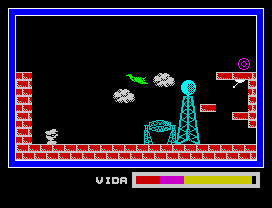
\includegraphics{../images/phantomas-sp1}
\caption{Phantomas (© 1986 Dinamic)}
\label{fig:phantomas}
\end{figure}

\bigskip
Todavía faltaba mucho tiempo para que aprendiera lo que era una interfaz (aún no había aprendido apenas a leer) pero ya sabía interpretar algunas letras, curiosamente las que tenían pintadas las teclas OPQA\footnote{En los primeros ordenadores de la década de los 80 OPQA era la combinación de teclas que usaban la mayoría de los juegos siendo OP las teclas para desplazarse de izquierda a derecha y QA para saltar o moverse de arriba a abajo.}.

\bigskip
Según fui creciendo aprendí a leer y escribir y también a diferenciar entre texto y código, para mí el código eran un serie de letras que aparecían impresas en las últimas páginas de las revistas que compraba mi hermano. Esos códigos se llamaban POKES\footnote{Instrucción en lenguaje BASIC para guardar un valor en una dirección de memoria.}, y cuando los introducías en un juego conseguías cosas como vidas infinitas, la habilidad de atravesar paredes o la capacidad de ser invisible a los enemigos. Sin saberlo estaba aprendiendo a programar de forma muy rudimentaria.

\bigskip
Algunos años mas tarde aparecieron las consolas de videojuegos en las que metías un cartucho e instantáneamente estabas jugando a juegos increíbles con una paleta de colores que raro era que no provocara ataques epilépticos. Mientras mis amigos solo tenían que introducir el cartucho y empezar a jugar yo tenía que esperar 5 interminables minutos mientras escuchaba sonidos estridentes y cruzar los dedos por que no apareciera el fastidioso TAPE ERROR que se podía intentar solucionar girando un tornillo llamado ``azimut'' con un destornillador de estrella.

\bigskip
Y de esta manera, sin siquiera saberlo, tuve mis primeros contactos con el auto-aprendizaje, yo girando un tornillo sin saber a ciencia cierta el por qué y cuando el mayor problema que tenían mis amigos era que a veces tenían que dar un soplido fuerte al cartucho.

\bigskip
Pasaron los años, los sistemas se fueron haciendo mas complejos y me di cuenta de que cuantas más opciones tenían los dispositivos, más perezosos se volvían los usuarios. Mi vecino sin ir más lejos, por no aprender a ajustar su televisor tenía ``La 2'' en el canal 3 ¿era yo el único que encontraba eso chirriante? Quizá no, pero como he ido descubriendo hay diferentes tipos de personas, están los que pueden pasar meses alumbrando el pasillo con el teléfono móvil y los que crean un tutorial en YouTube para enseñar a cambiar una bombilla.

\bigskip
Y ese es el deber que tenemos como futuros profesores, ser capaces de transmitir ese conocimiento e intentar que nuestros alumnos no pasen meses a oscuras, que aprendan a silenciar el volumen del altavoz del módem y en el mejor de los casos que sepamos despertar en ellos la curiosidad para que sean ellos mismos los que auto-aprendan y descubran todas esas cosas futuras que aun siendo profesores tenemos por aprender.

\section{Análisis general del problema}

La enseñanza de la programación suele considerarse bastante complicada, ``ya que muchos estudiantes encuentran bastantes dificultades cuando empiezan a programar'' (\cite{rubio_uso_2018}), de hecho ``la existencia de altas tasas de fracaso y la subsiguiente incapacidad de los estudiantes para escribir programas simples al final de una unidad de programación son solo dos de los problemas que inciden en las facultades de informática todo el mundo'' (\cite{bruce_contemporary_nodate}).

\bigskip
Aun así la programación es uno de los pilares más importantes de la informática, por lo que su aprendizaje es de carácter obligatorio. De hecho en muchos países como Finlandia, Alemania y Estonia promueven el aprendizaje de programación desde la educación primaria, en nuestro país \textit{``el estudio de las CC en Educación Primaria y Secundaria se encuentra en su fase inicial y se ha empezado a introducir recientemente por lo que aún no ha sido adoptado por la mayoría de centros escolares. Como resultado, el número de niños y niñas que a día de hoy estudian ciencias de la computación es todavía una minoría''} (\cite{fecyt_educacion_2016}) pero se está promoviendo el aprendizaje a edades cada vez más tempranas.

\bigskip
Para enseñar programación a nuestros alumnos tenemos que tener en cuenta las dificultades que suponen la interacción ordenador/alumno y ``contar con una actitud receptiva a los problemas que les plantea a los alumnos la introducción de un lenguaje formal y su uso para programar y resolver problemas''(\cite{vitale_psycopedagogical_1990}).


% No me cuadra tener una lista de objetivos aquí y otra en la sección 2 y encima que no sean los mismos... Mejor describe el problema en párrafos. Aprovecha para explicar por qué es necesario en programación que los estudiantes practiquen mucho, cómo el profesor no podrá nunca corregir todos los ejercicios que permitirían una práctica intensiva, que le uso de esta herramienta facilita al estudiante probar, ver en qué se equivoca, corregir y muy sucintamente qué beneficios aporta al profesor aparte del ahorro de tiempo... todo lo que justifique abordar el problema que abordas en tu TFM

% Echa un ojo a lo que te he puesto en la sección 4.1


% Veo muy floja la descripción del problema, puedes contar muchas cosas más, cuenta también la forma en la que se enseña actualmente, los problemas que tiene, etc. Tienes que darle una buena vuelta. Llévate este apartado a la sección 1.2


Este proyecto intentará abordar los siguientes objetivos:

\section{Estructura del proyecto}

\bigskip
Antes de pasar a detalles más técnicos, me gustaría detallar el contenido de este proyecto:

\begin{itemize}
  \item En el \textit{capítulo 1} (\textbf{Introducción}) se encuentra una breve introducción a nuestra idea, así como las motivaciones que nos han llevado a realizarla.
  \item El \textit{capítulo 2} (\textbf{Objetivos}) define los objetivos que se quieren alcanzar con este proyecto.
  \item En el \textit{capítulo 3} (\textbf{Antecedentes}) se analiza el estado de arte actual, así como algunas de las tecnologías y paradigmas que utilizaremos en nuestro proyecto.
  \item En el \textit{capítulo 4} (\textbf{Propuesta pedagógica}) se analizan los detalles pedagógicos del proyecto.
  \item En el \textit{capítulo 5} (\textbf{Propuesta metodológica}) se planifica cómo se van a realizar de forma técnica los contenidos del proyecto.
  \item En el \textit{capítulo 6} (\textbf{Conclusiones}) se pueden encontrar las conclusiones finales así como las recomendaciones para futuros trabajos.

\end{itemize}


\bigskip
Para finalizar se incluye un anexo con el código fuente desarrollado y liberado bajo la licencia libre \cite{gplv3}. Dicho código fuente se puede encontrar en la url \url{https://github.com/erseco/ugr_tfm_maes_sample_exercises/}.


% %
% % Ejemplos de codigo LaTeX para uso futuro
% %

% \begin{figure}[h!]
% \centering
% 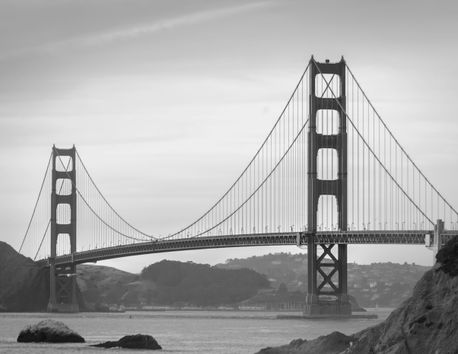
\includegraphics{../screenshots/sample1}
% \caption{Sample Image 1}
% \label{fig:sample1}
% \end{figure}

% Esto es un texto con una nota\footnote{Ejemplo de nota al pie} al pie.

% Y esto es una ``Frase de alguien''\cite{stevekrug}.

% \begin{itemize}
%   \item \textbf{1.} Texto de ejemplo
%   \item \textbf{2.} Texto de ejemplo
%   \item \textbf{3.} Texto de ejemplo
%   \item \textbf{4.} Texto de ejemplo

% \end{itemize}

% \begin{enumerate}
% 	\item Ejemplo 1.
% 	\item Ejemplo 2.
% \end{enumerate}

% \begin{lstlisting}[language=html]
% <!DOCTYPE html>
% <html lang="es-ES">
%   <head>
%     <meta charset="utf-8">
%     <title>Ejemplo de 2 párrafos</title>
%   </head>
%   <body>
%     <p>Esto es un párrafo.</p>
%     <p>Esto es otro párrafo.</p>
%   </body>
% </html>
% \end{lstlisting}

% Puedes verlo en \cite{Patricio2011}. Te recomiendo leer \cite{Patricio2011, Zacarias2009, Alfonso2010b, Alfonso2010a}.
